\documentclass{article}

\usepackage[margin=1in]{geometry}
\usepackage[pdfpagemode=UseNone,pdfstartview=]{hyperref}
\usepackage{booktabs,caption,csvsimple,graphicx,pdflscape}

\title{Term Yield Alternatives in FRED}
\author{Junyong Kim}
\date{September 8, 2020}

\begin{document}

\maketitle

\href{https://www.aeaweb.org/articles?id=10.1257/0002828043052240}{The Bad Beta Good Beta paper} uses $r_M^e$, $TY$, $PE$, and $VS$ as the state variables for its VAR model. The source of the author's original $TY$ is \href{http://www.globalfinancialdata.com/}{Global Financial Data}, which isn't publicly available. So I consider some publicly available alternative term yields from \href{https://fred.stlouisfed.org/}{Federal Reserve Economic Data}. I compare $TY$ and
\begin{itemize}
\item $t10yff$: \href{https://fred.stlouisfed.org/series/T10YFF}{10-Year Treasury Constant Maturity Minus Federal Funds Rate}
\item $t10y2y$: \href{https://fred.stlouisfed.org/series/T10Y2Y}{10-Year Treasury Constant Maturity Minus 2-Year Treasury Constant Maturity}
\item $t10y3m$: \href{https://fred.stlouisfed.org/series/T10Y3M}{10-Year Treasury Constant Maturity Minus 3-Month Treasury Constant Maturity}
\item $gs10gs5$: \href{https://fred.stlouisfed.org/series/GS10}{10-Year Treasury Constant Maturity Rate} minus \href{https://fred.stlouisfed.org/series/GS5}{5-Year Treasury Constant Maturity Rate}
\item $gs10gs3$: \href{https://fred.stlouisfed.org/series/GS10}{10-Year Treasury Constant Maturity Rate} minus \href{https://fred.stlouisfed.org/series/GS3}{3-Year Treasury Constant Maturity Rate}
\item $gs10gs2$: \href{https://fred.stlouisfed.org/series/GS10}{10-Year Treasury Constant Maturity Rate} minus \href{https://fred.stlouisfed.org/series/GS2}{2-Year Treasury Constant Maturity Rate}
\item $gs10gs1$: \href{https://fred.stlouisfed.org/series/GS10}{10-Year Treasury Constant Maturity Rate} minus \href{https://fred.stlouisfed.org/series/GS1}{1-Year Treasury Constant Maturity Rate}
\item $gs10gsm$: \href{https://fred.stlouisfed.org/series/GS10}{10-Year Treasury Constant Maturity Rate} minus the mean of \href{https://fred.stlouisfed.org/series/GS3}{3-Year Treasury Constant Maturity Rate} and \href{https://fred.stlouisfed.org/series/GS1}{1-Year Treasury Constant Maturity Rate}
\item $gs10dgs3mo$: \href{https://fred.stlouisfed.org/series/GS10}{10-Year Treasury Constant Maturity Rate} minus \href{https://fred.stlouisfed.org/series/DGS3MO}{3-Month Treasury Constant Maturity Rate}
\end{itemize}
based on their descriptive statistics, correlations, and historical behavior.

The results show that both $t10y2y$ and $gs10gs2$ have the higest correlations of 0.91 with $ty$. However, $gs10gsm$, which starts in April 1953, has 278 more observations than $gs10gs2$, which starts in June 1976.

The SAS code downloads the data and computes the numbers.

\begin{landscape}
\begin{table}
\centering
\caption*{Descriptive statistics from $TY$ and its alternatives}
\csvautobooktabular{means.csv}
\end{table}

\begin{table}
\centering
\caption*{Correlations between $TY$ and its alternatives}
\csvautobooktabular{corr.csv}
\end{table}
\end{landscape}

\noindent
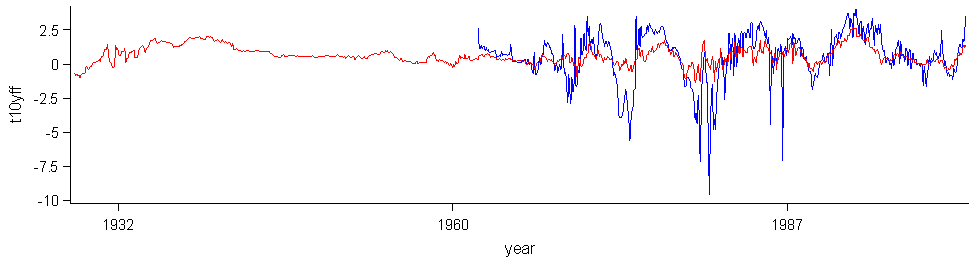
\includegraphics{series/t10yff}\\
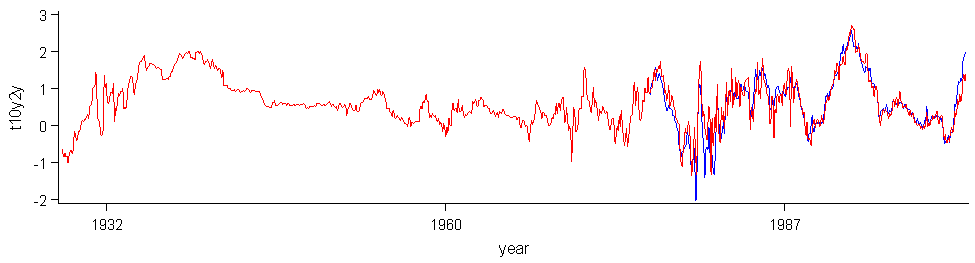
\includegraphics{series/t10y2y}\\
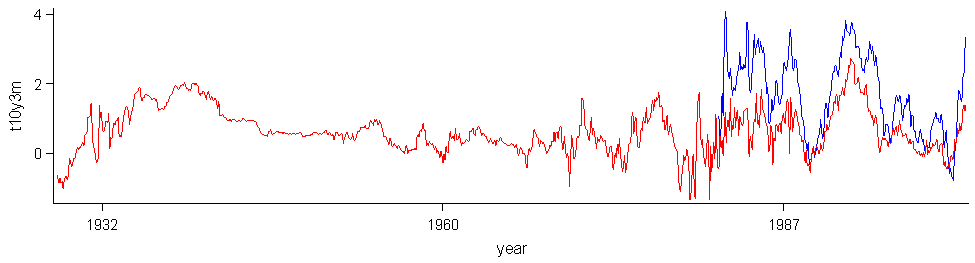
\includegraphics{series/t10y3m}\\
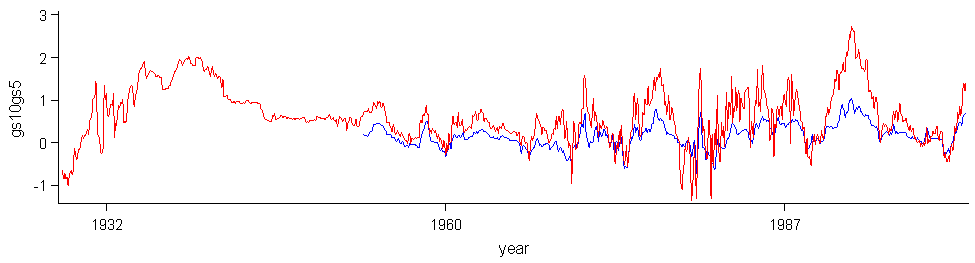
\includegraphics{series/gs10gs5}\\
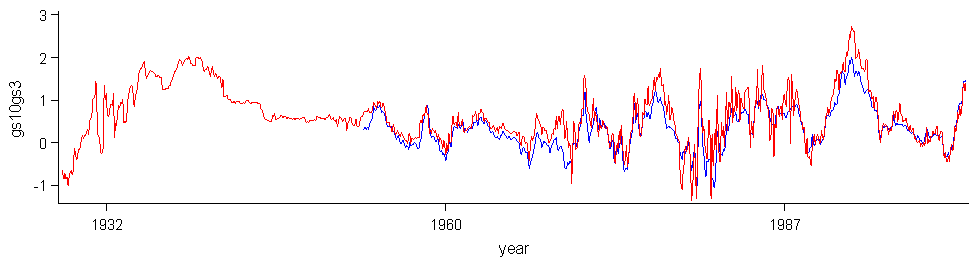
\includegraphics{series/gs10gs3}
\clearpage

\noindent
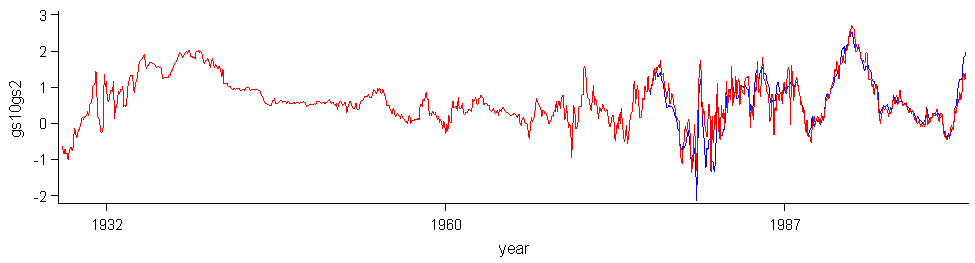
\includegraphics{series/gs10gs2}\\
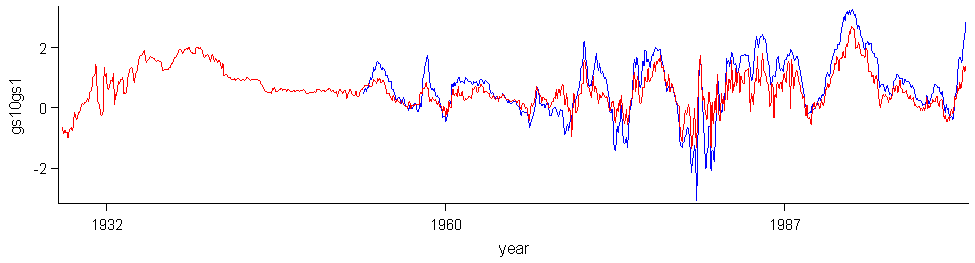
\includegraphics{series/gs10gs1}\\
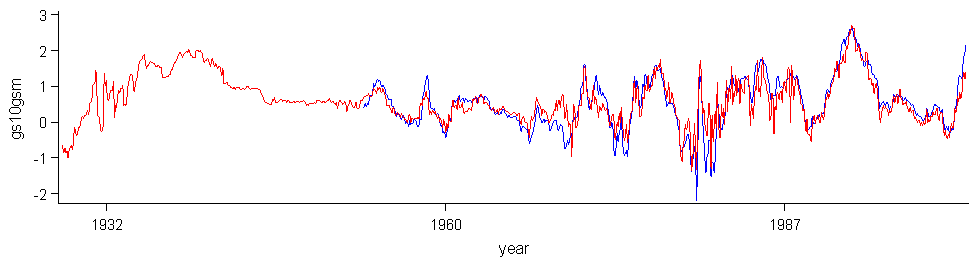
\includegraphics{series/gs10gsm}\\
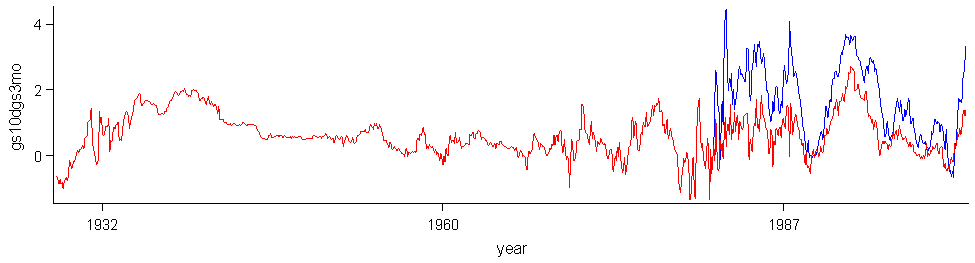
\includegraphics{series/gs10dgs3mo}
\clearpage

\noindent
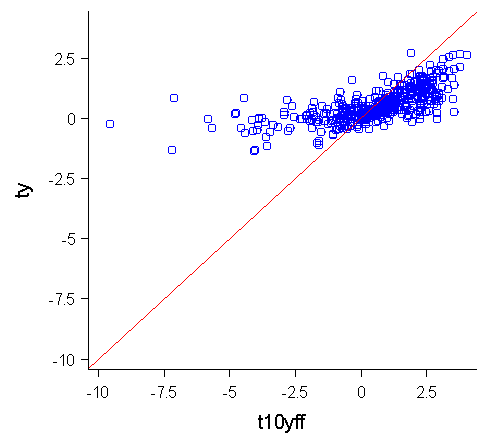
\includegraphics{scatter/t10yff}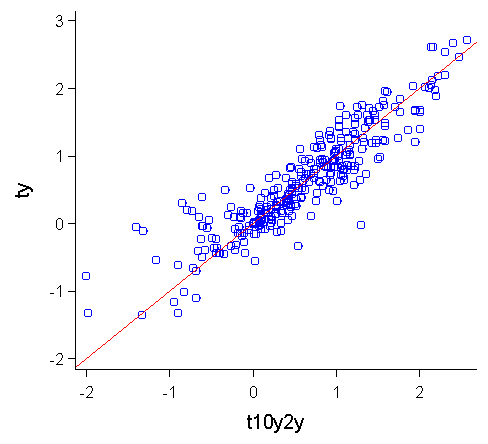
\includegraphics{scatter/t10y2y}\\
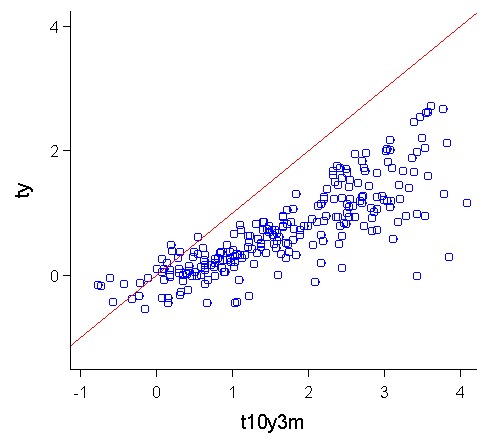
\includegraphics{scatter/t10y3m}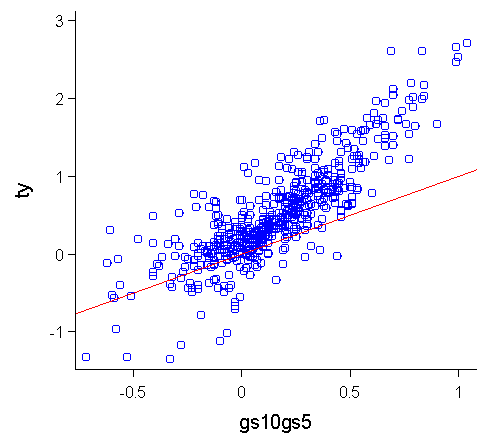
\includegraphics{scatter/gs10gs5}\\
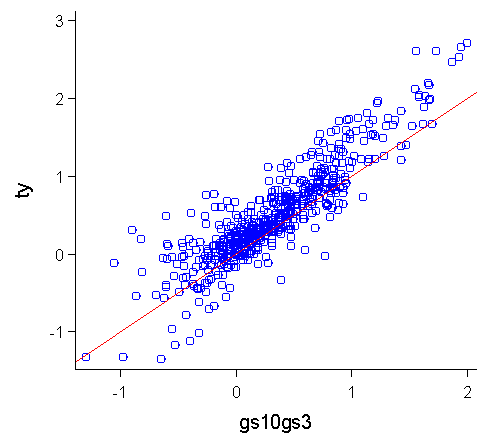
\includegraphics{scatter/gs10gs3}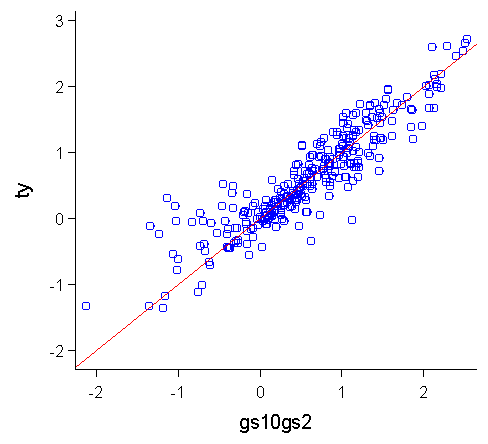
\includegraphics{scatter/gs10gs2}
\clearpage

\noindent
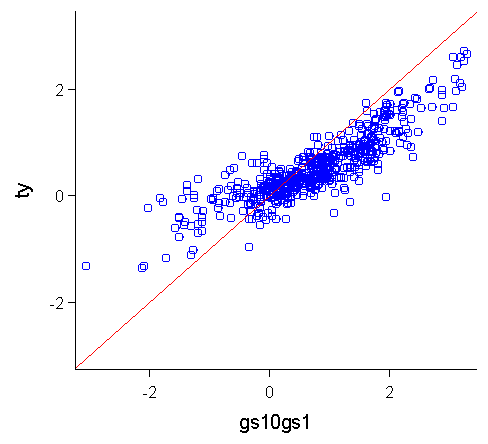
\includegraphics{scatter/gs10gs1}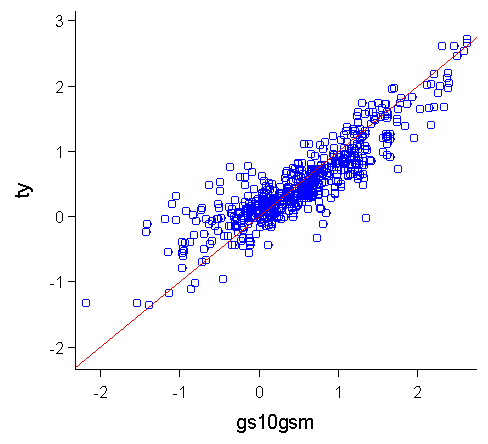
\includegraphics{scatter/gs10gsm}\\
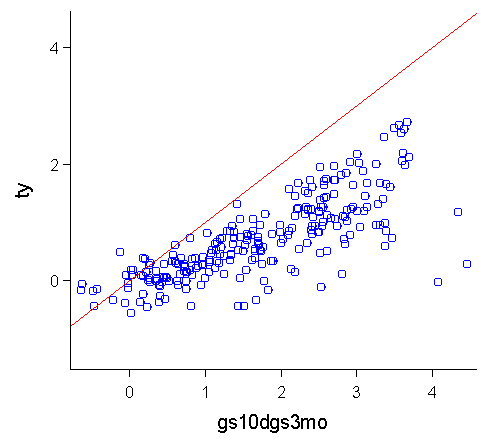
\includegraphics{scatter/gs10dgs3mo}

\end{document}
